\begin{frame}{Planificación}
  \textbf{Desarrollo iterativo.} \pause
  \begin{enumerate}
  \item Adquisición de base de conocimientos. \pause
  \item Desarrollo de analizador básico. \pause
  \item Interfaz gráfica de usuario. \pause
  \item Motor de lecciones. \pause
  \item Motor de canciones. \pause
  \end{enumerate}
\end{frame}

{
  \setbeamertemplate{background}{
\includegraphics[width=\paperwidth,height=\paperheight]{imagenes/fondo_simple.pdf}}
  \begin{frame}{Diagrama de Gantt}
    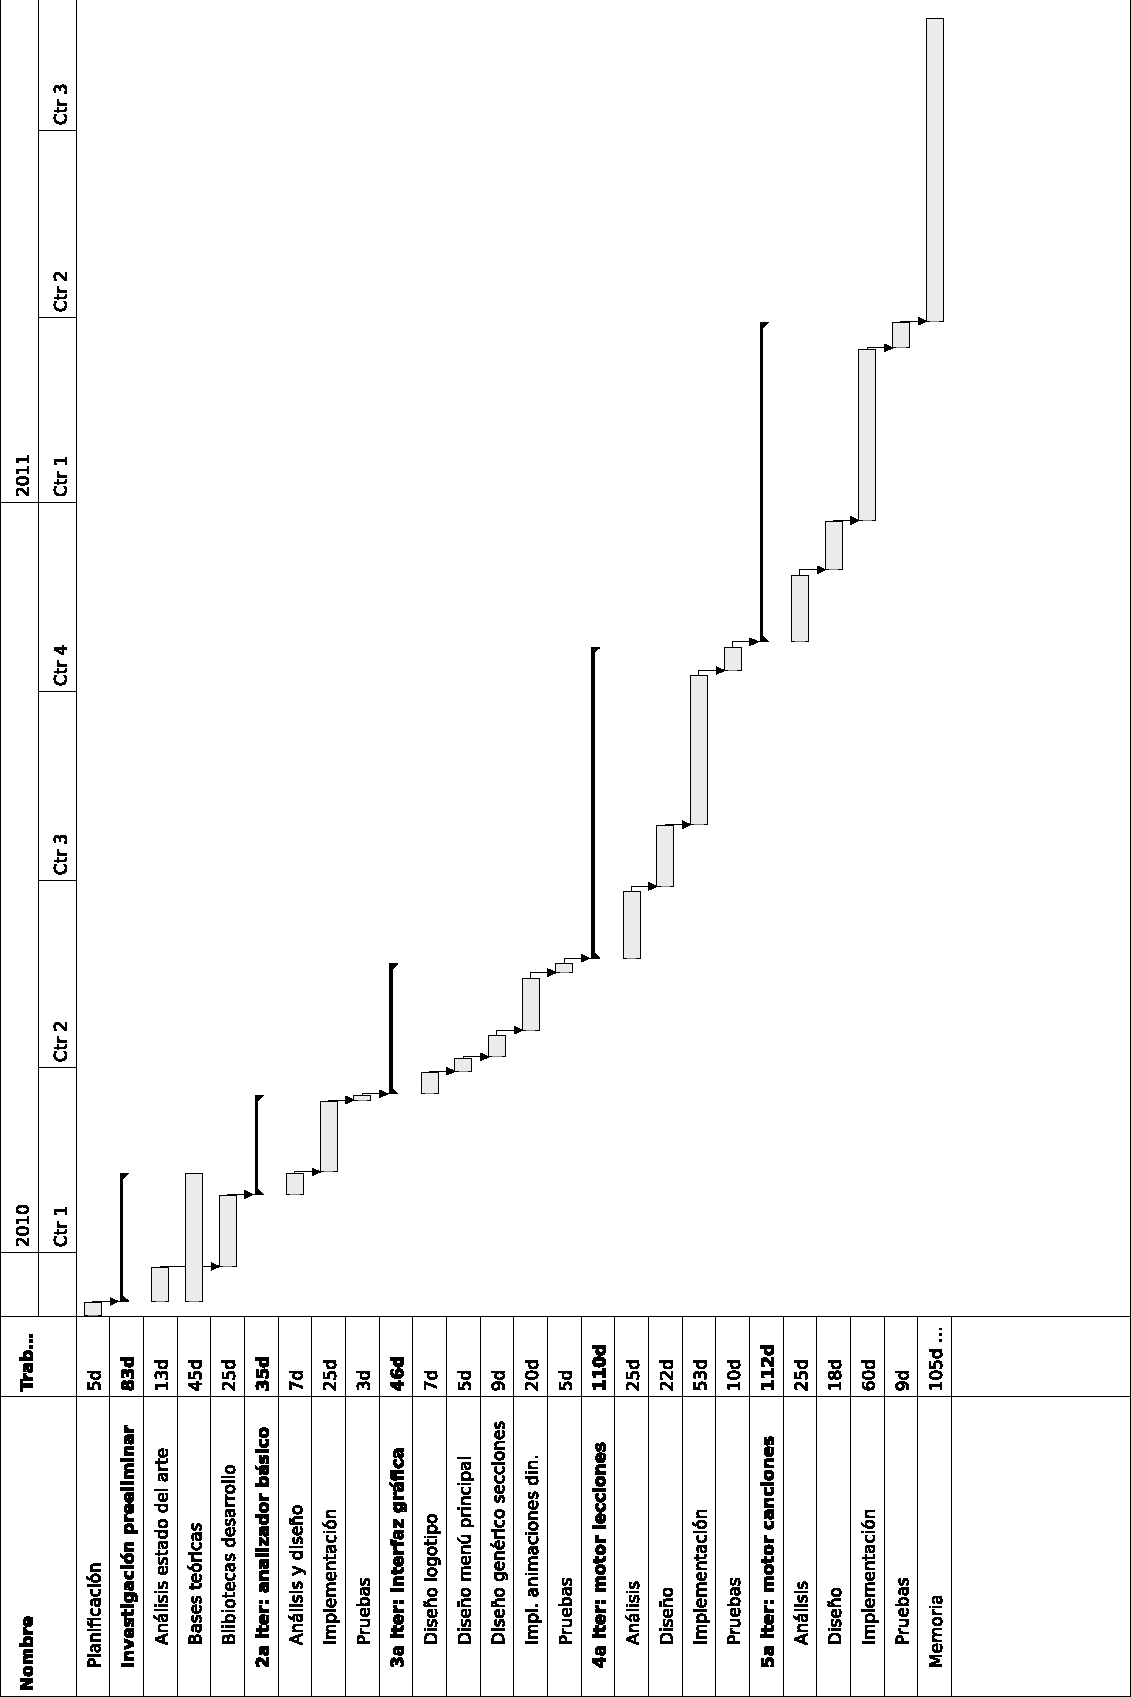
\includegraphics[angle=270, width=\textwidth]{imagenes/imagen_diagrama_gantt}
  \end{frame}
}

%%% Local Variables: 
%%% mode: latex
%%% TeX-master: "../presentacion"
%%% End: 
